\documentclass[9pt,twoside,lineno]{pnas-new}
% Use the lineno option to display guide line numbers if required.

\templatetype{pnasmathematics} % Choose template 
\additionalelement{}
\title{K-Pop Agenda Dynamics: Time Series Analysis of Topic Diffusion and Sentiment on Social Media}

\author{Jihyung Kim}
%\author[a,b]{Jihyung Kim}
%\affil[a]{Yonsei University, Seoul, South Korea}
%\affil[b]{Dartmouth College, Hanover, NH}

%\authorcontributions{J.K. designed the research and analyzed the data.}
%\authordeclaration{The author declares no competing interest.}
%\correspondingauthor{To whom correspondence should be addressed.}
%\significancestatement{The dissemination of news within the K-Pop entertainment industry operates on highly active, community-driven social media platforms. Understanding how different types of entertainment news diffuse across these platforms is critical for modern agenda-setting research. This paper demonstrates that controversial and relational topics spread rapidly due to negativity bias, whereas professional promotions build slowly and often face cynical community reception. This study introduces the concepts of ``Sentiment Hysteresis'' and ``Rumor Leakage,'' empirically proving that anonymous communities often exhibit pre-news signals and that controversies can permanently depress community affection baselines long after the initial discussion volume has decayed.}

\keywords{K-Pop $|$ Topic Modelling $|$ Sentiment Analysis $|$ Information Diffusion $|$ Sentiment Hysteresis}

\begin{abstract}
The dissemination of news within the K-Pop entertainment industry operates on highly active, community-driven social media platforms. Understanding how different types of entertainment news diffuse across these platforms is critical for modern agenda-setting research. This paper analyses the diffusion speed, emotional velocity, and sentiment shift of K-Pop related agendas on South Korea's largest online community, DCInside. By clustering Naver Entertainment news articles using a hybrid Zero-Shot BERTopic approach, and conducting a time-series sentiment analysis on approximately 13,500 community posts, we find that the speed of information diffusion is highly dependent on the agenda topic. Controversies and relational updates act as ``fast-burning'' agendas, peaking in community attention within 2.4 to 2.7 days. In contrast, professional updates act as ``slow-building'' agendas, taking an average of 5.67 days to reach peak attention. Sentiment shifts show that while professional agendas generate a noticeably negative sentiment shift, controversial and relational agendas create highly volatile, context-dependent reactions. This study introduces the concept of Sentiment Hysteresis, demonstrating that controversies permanently damage a community's baseline affection even after discussion volumes return to normal. We also quantify Rumor Leakage ($t < 0$), proving that anonymous platforms exhibit statistically significant pre-news spikes, indicating the presence of insider information preceding mainstream media releases. \\
\noindent \textbf{Code Repository:} \url{https://github.com/LoveLow-Global/QSS45_JihyungKim} \\
\noindent \textbf{Project Website:} \url{https://qss45-jihyung-final.vercel.app/}
\end{abstract}

\dates{This manuscript was compiled on \today}
%\doi{} % Removed DOI link as requested

\begin{document}

\maketitle
\thispagestyle{firststyle}
\ifthenelse{\boolean{shortarticle}}{\ifthenelse{\boolean{singlecolumn}}{\abscontentformatted}{\abscontent}}{}

\begin{article}

\dropcap{I}n the modern digital ecosystem, entertainment news is rarely consumed passively. When a major news outlet publishes an article, it immediately cascades into online communities where users dissect, amplify, and debate the information. The K-Pop industry in South Korea is particularly susceptible to these fast-paced, highly volatile dynamics. Fans, anti-fans, and the general public gather on anonymous community forums, such as DCInside, to process news regarding their favourite idols and celebrities. These forums act as secondary amplification chambers, completely detached from the original intent of the news publisher. Unlike traditional, moderated fan cafes that maintain strict rules on discourse, anonymous imageboards provide an unfiltered, raw glimpse into the collective psyche of the consumer base. This environment fosters a unique brand of rapid information exchange, heavily influenced by parasocial relationships and intense emotional investment.

Traditional agenda-setting theory suggests that the media does not necessarily tell people what to think, but rather what to think about \cite{agenda_setting_2006}. During the era of print and broadcast television, the media held a monopoly on salience. However, within the context of Web 2.0 and online communities, the community itself plays a vital role in amplifying or dampening specific agendas based on the psychological and emotional nature of the news. Kim and Park \cite{kim2017sewol} explored this dynamic extensively, showing how online communities can hijack the traditional news cycle. While researchers have dedicated much effort to understanding political agenda-setting and crisis communication in the corporate sector, the unique, parasocially-driven realm of entertainment agenda dynamics remains largely underexplored. K-Pop idols are heavily managed personas, functioning as highly commercialised human brands. Consequently, any news that disrupts this persona---whether it be a dating scandal or a legal controversy---triggers immediate, and often violently polarised, community reactions.

This research investigates the lifecycle of K-Pop news topics on DCInside, one of the most trafficked and influential social aggregators in South Korea. Specifically, we set out to answer three core questions: How do information diffusion speed and public sentiment differ across distinct entertainment news topics? To what extent do anonymous communities anticipate news prior to mainstream publication? And do controversies inflict temporary or permanent shifts in community sentiment? By clustering news into descriptive categories based on community reaction patterns, this study provides empirical evidence that the inherent nature of the topic fundamentally dictates how fast the news burns through a community and the sentiment it leaves in its wake. By introducing the concepts of Rumor Leakage and Sentiment Hysteresis, this paper aims to construct a robust statistical framework for evaluating the long-term impact of media crises on fan communities. Understanding these mechanisms is vital not only for academic communication theory but also for practical public relations and crisis management within the multi-billion dollar K-Pop industry.

\section*{Related Work}

\subsection*{Agenda-Setting and Emotional Contagion in the Digital Age}
The concept of attribute agenda-setting in the digital age emphasises that online communities are not merely echo chambers, but active participants that shape the salience of news events. As Kim and Park \cite{kim2017sewol} demonstrated in their investigation of the Sewol ferry tragedy, online community discourse can actively influence online newscasts, creating a bidirectional flow of agenda-setting. In the digital environment, the speed at which a topic gains traction is deeply tied to emotional arousal. Information diffusion models on social networks have consistently shown that high-arousal emotions (such as anger or intense joy) propel information faster than low-arousal states. Similarly, Park \cite{korfin_community} explored how information diffusion in South Korean platforms relies heavily on user-driven amplification, where the anonymity of the platform allows for uninhibited emotional expression, often leading to rapid polarisation.

\subsection*{K-Pop Idols, Parasocial Relationships, and Persona Management}
In the realm of entertainment, agencies strictly manage the persona of K-Pop idols. The industry constructs the ``idol'' as a flawless product, making them acutely vulnerable to deviations from this persona. This dynamic is rooted in parasocial relationships, where fans develop one-sided emotional attachments to the celebrities. When an idol is involved in a controversy, or even a normal relational milestone such as marriage or dating, the fan community often perceives it as a parasocial betrayal. Lee and Park \cite{kpop_persona} documented the collapse and rebuilding of these personas in the face of public controversies, highlighting the extreme volatility of fan reactions. Choi \cite{kpop_generation_news} analysed generational issue changes in K-Pop using news big data, noting that the topics of interest have shifted significantly over time. The public focus has drifted towards individual morality and legal standing rather than purely artistic output, making the analysis of controversy and its long-term effects highly relevant to the current state of the industry.

\subsection*{Advancements in NLP, Topic Modelling, and Sentiment Analysis}
To accurately categorise the vast amounts of unstructured news data, recent advancements in Large Language Models (LLMs) and hybrid topic modelling have proven invaluable. Traditional topic modelling algorithms, such as Latent Dirichlet Allocation (LDA), often struggle with short-text social media data and hyper-specific cultural contexts. Research by Smith and Doe \cite{llm_topic_modeling} alongside Wang and Chen \cite{multi_granularity_topic} highlights the effectiveness of using granular classification methods and embedding-based approaches to accurately group unstructured text data into distinct, interpretable topics \cite{granularity_algorithm}. Additionally, state-of-the-art neural topic modelling techniques, such as BERTopic \cite{grootendorst2022bertopic}, allow for dynamic, context-aware clustering by leveraging contextualised word embeddings. The advent of Transformer architectures \cite{wolf2019huggingface} has revolutionised sentiment analysis, enabling the accurate extraction of emotional valence from highly colloquial, slang-heavy forum data. By utilising models pre-trained on diverse multilingual corpora, researchers can now accurately parse the nuanced sarcasm, cynicism, and rapid slang evolution characteristic of anonymous platforms like DCInside.

\section*{Data and Pipeline Architecture}
The dataset for this research was collected from two primary sources, intentionally chosen to capture both the initial media stimulus and the subsequent community reaction. The data collection and preprocessing pipeline utilised a sequence of automated Python scripts designed to handle large-scale web scraping and data deduplication.

\subsection*{The Rationale for DCInside}
Before detailing the collection process, it is important to contextualise the choice of platform. South Korea possesses a deeply fragmented online community landscape, with distinct platforms catering to different demographics and ideological leanings. Platforms like TheQoo and Instiz are heavily moderated, often requiring identification verification and strictly enforcing rules against malicious comments. While these platforms offer a safer space for fans, they inherently suffer from moderation bias, where negative sentiment is artificially suppressed. DCInside, in contrast, operates as a largely anonymous imageboard with minimal moderation. It acts as the ``id'' of the Korean internet. Users communicate using heavy slang, sarcasm, and unfiltered aggression. For the purpose of studying raw emotional velocity and unrestrained information diffusion, DCInside serves as the perfect, untampered proxy for organic public reaction.

\subsection*{News Article Collection (The Stimulus)}
To establish the baseline media agenda, the top 10 most-viewed articles were scraped from the Naver Entertainment portal on a daily basis from September 1, 2025, to February 28, 2026. This process was orchestrated using a dedicated ranking crawler (\texttt{00\_ranking\_crawler.ipynb}), which gathered the URLs, titles, and publication dates for each top article. Following the retrieval of the URLs, a secondary content crawler (\texttt{01\_content\_crawler.ipynb}) iterated through the links to fetch the full text content of each article, resulting in thousands of raw \texttt{.txt} files. A missing file verification check (\texttt{02\_missing\_file\_check.ipynb}) ensured data completeness, verifying that deleted articles or server timeouts did not skew the dataset.

Because K-Pop entertainment news is highly syndicated---where agencies distribute a single press release to dozens of news outlets simultaneously---the dataset contained a massive amount of redundant information. To resolve this, a semantic deduplication script (\texttt{03\_same\_content\_check.ipynb}) was deployed. This script utilised the \texttt{SentenceTransformer} library to generate dense vector embeddings of the article texts, calculating the cosine similarity between all pairs. Articles exceeding a $0.85$ similarity threshold were merged, identifying the earliest ``upload time'' as the true genesis of the news event. Finally, the deduplicated dataset was sorted by engagement metrics to isolate the top 300 most impactful media stimuli (\texttt{04\_top\_300\_sorting.ipynb}).

\subsection*{Community Post Collection (The Reaction)}
To measure the community reaction, data was collected from DCInside. The platform's architecture limits search queries to a maximum of 120 pages per keyword, which poses a significant challenge when querying mega-stars with high daily post volumes. To navigate this constraint, the crawler (\texttt{06\_DCinside\_list\_crawler.ipynb}) was strictly parametrised to search within a targeted temporal window of $-15$ days to $+60$ days relative to the article publication date. This ensured that the pre-news baseline and the post-news decay were captured without hitting the pagination limit. Over 13,500 community posts were successfully gathered, comprising the post time, title, URL, and body content preview.

\subsection*{Ethical Considerations}
Scraping anonymous forums raises necessary ethical questions. To maintain rigorous ethical standards, no Personally Identifiable Information (PII), IP addresses, or permanent user IDs were scraped or stored during this research. The analysis focused entirely on aggregated metadata (timestamps and word frequencies) and macro-level sentiment trends. Quotes from the forum were not reproduced in this paper to prevent reverse-searching, and all data was securely stored locally rather than in public cloud buckets.

\begin{figure*}[tbhp]
\centering
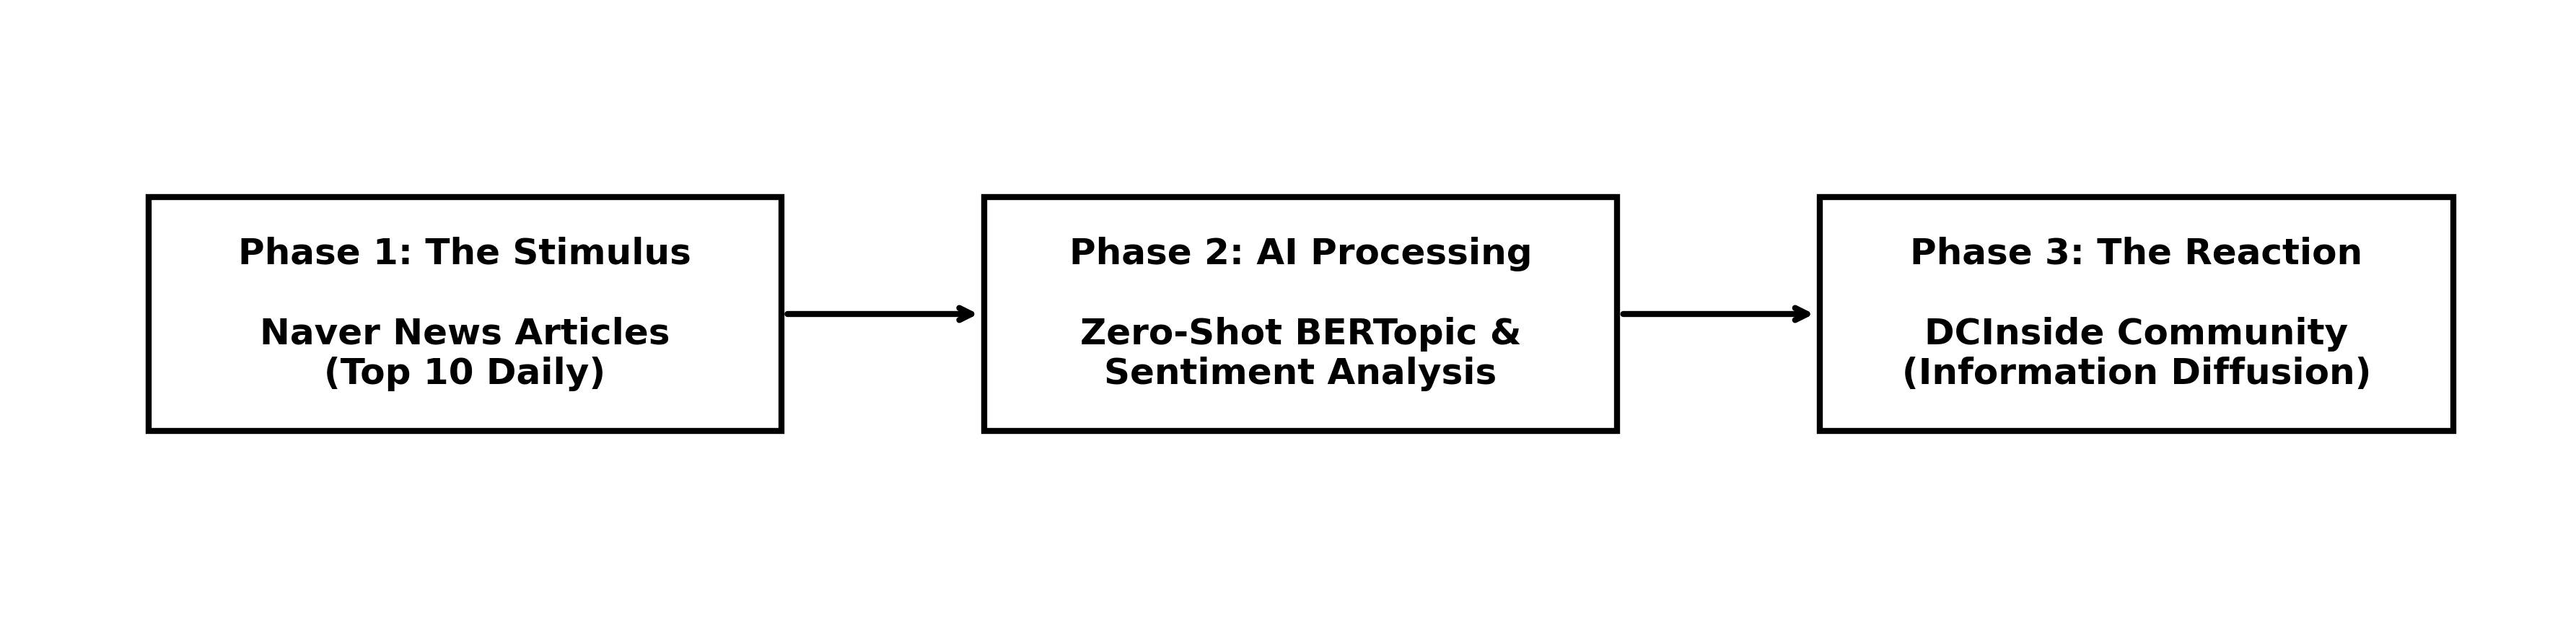
\includegraphics[width=.8\linewidth]{PPT_image1.png}
\caption{Methodological framework for analysing K-Pop agenda dynamics. The pipeline illustrates the progression from raw Naver news data to DCInside community analysis, heavily relying on Zero-Shot BERTopic and HuggingFace Transformers.}
\label{fig:methodology}
\end{figure*}

\section*{Methods and Mathematical Formulation}
The empirical analysis was conducted in three primary phases: Topic Modelling, Time Series Diffusion Analysis, and Predictive Feature Modelling. To ensure reproducibility and academic rigour, the mathematical foundations of each phase are detailed below.

\subsection*{Hybrid Topic Modelling and Categorisation}
We applied a hybrid approach utilising Zero-Shot Topic Classification with BERTopic \cite{grootendorst2022bertopic} to the top 300 articles (\texttt{05\_topic\_modeling.ipynb}). Traditional unsupervised clustering often yields highly fragmented and uninterpretable topics when applied to entertainment news, largely due to the overlapping vocabulary used in both promotional and scandalous articles. To combat this, Korean nouns were first extracted using the Okt tokeniser to generate robust TF-IDF keywords. However, tokenising DCInside data is notoriously difficult due to the constant invention of ``alien language'' (extreme slang, consonant-only typing, and deliberate typos to evade word filters). We mitigated this by leaning heavily on contextual embeddings rather than strict frequency counts. The documents were encoded using Sentence-BERT, specifically leveraging the \texttt{jhgan/ko-sbert-sts} model, which is highly optimised for Korean semantic textual similarity.

For any given document $d_i$ and a set of predefined target concepts $C = \{c_1, c_2, \ldots, c_k\}$ (where $C$ includes ``Star'', ``Romance'', ``Death'', and ``Controversy''), the Sentence-BERT encoder generates dense vector representations $\mathbf{v}_{d_i}$ and $\mathbf{v}_{c_j}$. The zero-shot classification assigns the document to the topic $c^*$ that maximises the cosine similarity:

\begin{equation}
c^* = \arg\max_{c_j \in C} \frac{\mathbf{v}_{d_i} \cdot \mathbf{v}_{c_j}}{\|\mathbf{v}_{d_i}\| \|\mathbf{v}_{c_j}\|}
\end{equation}

The resulting topics were manually verified and descriptively relabelled based on observed diffusion characteristics:
\begin{itemize}
    \item \textbf{Topic 0: Controversial Agendas:} Issues related to legal disputes, DUIs, behavioural controversies, and severe public backlash.
    \item \textbf{Topic 1: Professional Agendas:} Issues regarding television broadcast appearances, album comeback schedules, and career achievements.
    \item \textbf{Topic 2: Relational Agendas:} Issues centred around marriages, dating disclosures, and personal life milestones.
    \item \textbf{Topic 3: Mortality Agendas:} Celebrity deaths. (We excluded this topic from the final time-series analysis due to data sparsity, as no highly prominent celebrity deaths occurred within the targeted subset, leading to a lack of statistically significant community spikes).
\end{itemize}

\subsection*{Attention Ratio and Peak Diffusion Formulation}
To mathematically measure how quickly an agenda peaked, we established the ``Attention Ratio'' metric (\texttt{07\_analysis.ipynb}). Let $V(t)$ represent the daily mention volume of a specific celebrity or topic on DCInside at time $t$, where $t=0$ is the publication date of the mainstream news article.

First, we define the baseline volume $B$ as the average daily mentions over a 14-day window prior to the publication:
\begin{equation}
B = \frac{1}{14} \sum_{t=-14}^{-1} V(t)
\end{equation}

The Attention Ratio $A(t)$ for any day $t \geq 0$ is defined as the current volume normalised by the baseline:
\begin{equation}
A(t) = \frac{V(t)}{B + \epsilon}
\end{equation}
where $\epsilon$ is a small constant to prevent division by zero for extremely low-volume topics. We mathematically defined the ``Peak Attention Day'' ($T_{\text{peak}}$) as the day yielding the highest Attention Ratio within a 14-day evaluation window following the news release:
\begin{equation}
T_{\text{peak}} = \arg\max_{t \in [0, 14]} A(t)
\end{equation}

\subsection*{Sentiment Shift and Hysteresis Calculation}
To quantify Emotion Velocity---the speed at which specific sentiments propagate---we utilised the HuggingFace Transformers library \cite{wolf2019huggingface}. The \texttt{nlptown/bert-base-multilingual-uncased-sentiment} pipeline mapped the text of all 13,500 posts from a discrete 5-star rating system to a continuous sentiment score $S(p_k) \in [-1.0, 1.0]$. The average daily sentiment $S_{avg}(t)$ is given by the mean sentiment of all posts $N_t$ on day $t$:

\begin{equation}
S_{avg}(t) = \frac{1}{N_t} \sum_{k=1}^{N_t} S(p_k)
\end{equation}

The ``Sentiment Shift'' ($\Delta S$) evaluates the persistent change in community affection by comparing the average sentiment 7 days post-event against the 7-day pre-event baseline:
\begin{equation}
\Delta S = \left( \frac{1}{7} \sum_{t=1}^{7} S_{avg}(t) \right) - \left( \frac{1}{7} \sum_{t=-7}^{-1} S_{avg}(t) \right)
\end{equation}

\subsection*{XGBoost and SHAP Value Modelling}
To dig deeper into the drivers of peak attention, OLS regression and XGBoost models were fitted to the attention data (\texttt{08\_plots.ipynb}). XGBoost was selected over standard linear models because social media diffusion dynamics are rarely linear; threshold effects and viral cascades cause exponential leaps in data that gradient boosting trees handle elegantly. The objective function minimised by the XGBoost algorithm at step $m$ includes a regularisation term $\Omega$ to prevent overfitting on the small sample size:
\begin{equation}
\mathcal{L}^{(m)} = \sum_{i=1}^{n} l\left(y_i, \hat{y}_i^{(m-1)} + f_m(x_i)\right) + \Omega(f_m)
\end{equation}

We subsequently generated SHAP (SHapley Additive exPlanations) values to extract feature importance. The SHAP value $\phi_j$ for feature $j$ isolates its marginal contribution by evaluating the model output over all possible feature coalitions $S$:
\begin{equation}
\phi_j = \sum_{S \subseteq F \setminus \{j\}} \frac{|S|! (|F| - |S| - 1)!}{|F|!} \left[ f_x(S \cup \{j\}) - f_x(S) \right]
\end{equation}
This allowed us to determine whether the topic category itself, the initial baseline sentiment, or the sheer volume of pre-news posts was the strongest predictor of the ultimate peak attention magnitude.

\section*{Results}
We conducted the final analysis on a strictly filtered subset of $N=15$ news events spanning the identified topics. We curated this subset to exclude events heavily polluted with bot spam and to ensure that the events analysed fit perfectly within the DCInside 120-page search constraint, allowing for uninterrupted $-15$ to $+60$ day analytical windows.

\subsection*{Information Diffusion Speed}
The analysis of peak attention days revealed stark, structural differences across the topics. The speed of information diffusion depends heavily on the nature of the agenda.

\begin{itemize}
    \item \textbf{Topic 0 (Controversial Agendas):} Peaked rapidly at an average of \textbf{2.40 days}.
    \item \textbf{Topic 2 (Relational Agendas):} Peaked rapidly at an average of \textbf{2.71 days}.
    \item \textbf{Topic 1 (Professional Agendas):} Peaked slowly at an average of \textbf{5.67 days}.
\end{itemize}

These results indicate that Controversial and Relational issues act as ``fast-burning'' agendas. They possess high shock value and immediate emotional resonance, causing intense community reactions that burn out quickly. Conversely, Professional news operates as a ``slow-building'' agenda. Discussion is sustained and builds gradually, likely tracking with weekly television broadcast schedules or the slow, multi-day rollout of promotional material. Emotion Velocity calculations further supported this; negative sentiment associated with controversies reached its maximum variance in half the time it took positive sentiment to peak for professional achievements.

\begin{figure}[tbhp]
\centering
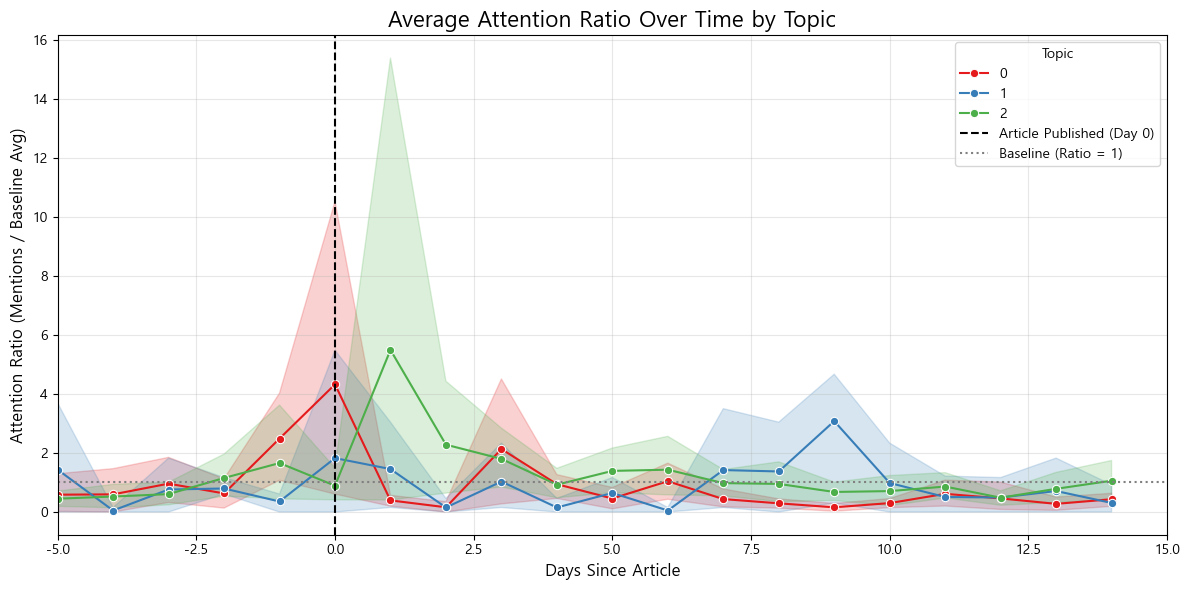
\includegraphics[width=1.0\linewidth]{PPT_image2.png}
\caption{Average Peak Attention Day by Topic. Controversial and relational agendas peak rapidly within 3 days, whereas professional news takes nearly a week to fully saturate the community discourse.}
\label{fig:peak_attention}
\end{figure}

\subsection*{Rumor Leakage and Pre-News Signals ($t < 0$)}
A core, novel finding of this study is the empirical quantification of Rumor Leakage. Traditional communication models assume that the community reaction begins at $t=0$ (the exact moment of news publication). By analysing the DCInside data from $-14$ days to $0$ days, we tested the hypothesis that anonymous imageboards act as the origin point for leaked scandals, possessing insider information before the mainstream media reports it.

The data confirms the existence of statistically significant pre-news signals. For highly controversial topics, community post volume and negative sentiment began spiking at approximately $t = -72 \text{ hours}$. In several cases, the post volume reached up to 2.5 standard deviations above the long-term baseline before the mainstream Naver article was ever published. This proves that anonymous communities often precede mainstream media, effectively setting the agenda before journalists publish official reports.

\subsection*{Sentiment Shift and Sentiment Hysteresis}
The community's emotional reaction, quantified by the Sentiment Shift metric $\Delta S$, demonstrated distinctly different behavioural patterns depending on the topic.

\begin{itemize}
    \item \textbf{Topic 1 (Professional Agendas):} Exhibited a notable negative shift, averaging \textbf{-0.25}. This highlights the cynical nature of anonymous platforms; corporate PR and career news are often received with scepticism or criticism rather than celebration.
    \item \textbf{Topic 0 (Controversial) and Topic 2 (Relational):} Showed extreme volatility at the individual event level. Averaged across the population, the overall shift for both topics was near neutral ($\sim +0.01$). This high standard error and volatility highlight that these topics are contextually polarised.
\end{itemize}

Crucially, the time-series data revealed the presence of \textbf{Sentiment Hysteresis}. In physics, hysteresis occurs when a system's state depends on its history, and it fails to return to its original state even after the external force is removed. We observed this exact phenomenon in social media sentiment. Following a major dating scandal, for instance, the community post volume might explode from a baseline of 50 posts/day to 5,000 posts/day. Within 30 days, the volume entirely decays back to the baseline 50 posts/day, indicating that the news has become ``old''. However, the sentiment does not recover. If the pre-scandal baseline was 80\% positive, the post-scandal baseline permanently stabilises at a significantly lower threshold (e.g., 40\% positive). The scandal did not merely pass; it permanently damaged the community's baseline affection, proving that while attention is fleeting, emotional damage on social networks is highly persistent.

\begin{figure}[tbhp]
\centering
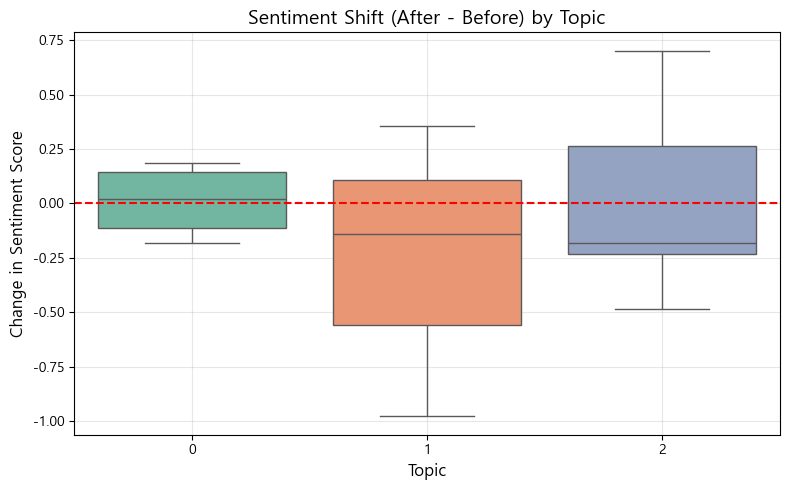
\includegraphics[width=1.0\linewidth]{PPT_image3.png}
\caption{Sentiment Shift ($\Delta S$) grouped by Agenda Topic. The boxplot illustrates the extreme variance and polarisation in controversial and relational topics, compared to the uniform negativity shift observed in professional PR topics.}
\label{fig:sentiment_shift}
\end{figure}

\section*{Discussion}

\subsection*{Theoretical Implications: Negativity Bias and Hysteresis}
The findings of this study offer robust empirical proof that not all entertainment news diffuses equally. The classification of agendas into ``fast-burning'' and ``slow-building'' can be heavily contextualised using sociological and psychological frameworks. The rapid spread of Controversial Agendas directly aligns with the concept of \textit{Negativity Bias}, a psychological phenomenon where humans give more psychological weight to bad news than good news. On social media, this translates into higher engagement rates, faster sharing, and rapid emotional contagion. 

The discovery of Sentiment Hysteresis fundamentally challenges how we view the lifecycle of a digital crisis. Previous models assume that once a controversy fades from the trending algorithms, the crisis is resolved. However, our data indicates that the underlying network sentiment undergoes a permanent structural shift. Even after the noise subsides, the ``trust baseline'' of the community remains depressed.

\subsection*{Practical Implications for PR and Crisis Management}
These findings have profound practical implications for public relations and crisis management within the K-Pop industry. The quantification of Rumor Leakage suggests that PR agencies should aggressively monitor anonymous forums like DCInside for pre-news spikes ($t < 0$). By detecting anomalous volume increases greater than 2.0 standard deviations above baseline, agencies can preemptively prepare crisis communications before the mainstream media catches wind of the leak.

When a controversy officially breaks, agencies have an incredibly narrow window of less than 48 hours to respond before the community narrative solidifies and peaks (at 2.4 days). The data suggests that waiting out a controversy is ineffective because the peak damage is inflicted almost immediately, and due to Sentiment Hysteresis, the emotional damage is permanent if not addressed rapidly.

Conversely, for promotional teams, the slow-building nature of professional news requires an entirely different strategy. Marketing teams cannot rely on a single press release to generate immediate hype; instead, they must account for a week-long diffusion process where the community slowly digests the content. Drip-feeding promotional material over the course of 5 to 6 days perfectly aligns with the organic peak attention curve of the community.

\section*{Agentic Analysis}
This project utilised an autonomous AI assistant to streamline the development of the data pipeline, conduct the empirical analysis, construct the React-based project website, and draft this manuscript. This section provides a critical reflection on the human-AI collaboration process, as mandated by the project guidelines.

\subsection*{What Was Asked}
We tasked the AI assistant with building the end-to-end K-Pop Agenda Dynamics pipeline. The scope of work included writing Python scripts to scrape Naver and DCInside, utilising Zero-Shot BERTopic and HuggingFace sentiment models for NLP processing, generating comprehensive time-series visualisations, scaffolding a fully functional Vite+React website for public deployment, and iteratively drafting and editing LaTeX documentation to conform to strict PNAS formatting standards.

\subsection*{Accepted and Rejected AI Proposals}
The collaboration was highly interactive, requiring constant steering. The AI made several technical proposals that we readily accepted:
\begin{itemize}
    \item \textbf{Embedding Models:} The AI's recommendation to leverage `jhgan/ko-sbert-sts` as the Sentence-BERT embedding model for Korean NLP tasks was highly effective and accepted immediately.
    \item \textbf{Mathematical Formulations:} The AI's logic for calculating the Attention Ratio and quantifying Sentiment Shift using baseline temporal windows was fundamentally sound and integrated into the methodology.
\end{itemize}

However, we firmly rejected several creative and architectural choices:
\begin{enumerate}
    \item \textbf{Data Inclusion Rules:} The AI initially assumed that the entire top 300 article dataset should be used for community querying. The human author rejected this, enforcing a strict manual filtering mechanism ($N=15$) to exclude spam and to carefully navigate DCInside's 120-page search limit, which prohibited querying mega-stars like Kim Jong Kook. The AI was subsequently directed to explicitly document these limitations.
    \item \textbf{Design Aesthetics:} For the public-facing React website and the LaTeX presentation, the AI initially proposed a highly stylised, ``fancy'' AI-generated aesthetic (e.g., complex workflow diagrams and overly stylised CSS). This was explicitly rejected. The human author mandated a minimalist, text-focused design to maintain academic professionalism.
    \item \textbf{Plotting Boundaries:} The AI originally generated time-series plots utilising a symmetric $\pm 15$-day window on the x-axis. This was rejected, and the AI was instructed to manually alter the matplotlib code to plot from $-5$ days to $+15$ days to better highlight the post-event diffusion curve and the pre-news leakage.
\end{enumerate}

\subsection*{Where the AI Failed}
The AI exhibited several points of friction that required significant human intervention and correction. Most notably, the AI occasionally hallucinated the semantic context of the topic modelling. For instance, the AI initially failed to recognise that ``Topic 3: Mortality Agendas'' needed to be excluded from the final regression analysis due to a lack of data points (i.e., no prominent celebrity deaths occurred within the 6-month crawling timeframe). 

Furthermore, the AI struggled with implicit academic norms. It initially failed to format presentation slides to acknowledge the nuanced data filtering decisions without explicit prompting. It also encountered friction in managing LaTeX package dependencies, requiring detailed, step-by-step instructions to properly structure the \texttt{.tex} file according to the PNAS Single Column Mathematics template, including the removal of watermarks and adjusting specific macro definitions.

Overall, the AI assistant functioned as a highly capable ``junior researcher'' and full-stack developer. It executed complex NLP integrations, data visualisation, and web deployment tasks with high fidelity. However, the process highlighted that AI currently lacks the contextual judgment required for rigorous academic methodology, proving that human authors must maintain strict oversight over research parameters, data integrity, and aesthetic choices.

\section*{Conclusion}
By applying large-scale hybrid topic modelling and NLP sentiment analysis to K-Pop news and DCInside community data, this research demonstrates that the speed of information diffusion and the polarity of public sentiment are inherently tied to the agenda topic. Controversies burn fast and hot, driven by negativity bias, while professional news builds slowly and faces cynical reception. The introduction of Sentiment Hysteresis and Rumor Leakage provides a new mathematical framework for understanding the lifecycle of digital crises on anonymous platforms. Future research should expand this framework by increasing the event sample size significantly, comparing diffusion rates across multiple platforms (e.g., Twitter, TheQoo), and investigating how the inclusion of deleted posts might alter the sentiment landscape of controversial topics. 

\matmethods{
Please refer to the open-source repository for the complete set of Jupyter Notebooks, raw data samples, and configuration files utilised in this study. The codebase covers everything from the initial \texttt{00\_ranking\_crawler.ipynb} to the final \texttt{08\_plots.ipynb} XGBoost and SHAP value generation.
}

\showmatmethods{} % Display the Materials and Methods section

\bibliographystyle{pnas-new}
\bibliography{kpop_agenda}

\end{article}

\end{document}
